\documentclass[conference]{IEEEtran}
\IEEEoverridecommandlockouts
% The preceding line is only needed to identify funding in the first footnote. If that is unneeded, please comment it out.
\usepackage{cite}
\usepackage{amsmath,amssymb,amsfonts}
\usepackage{algorithmic}
\usepackage{graphicx}
\usepackage{textcomp}
\usepackage{xcolor}
\def\BibTeX{{\rm B\kern-.05em{\sc i\kern-.025em b}\kern-.08em
    T\kern-.1667em\lower.7ex\hbox{E}\kern-.125emX}}
\begin{document}

\title{CENG466, Fall 2022, THE 1\\

}

\author{\IEEEauthorblockN{1\textsuperscript{st} Fırat Ağış}
\IEEEauthorblockA{\textit{Department of Computer Engineering} \\
\textit{Middle East Technical University}\\
Ankara, Turkey \\
e2236867@ceng.metu.edu.tr}
\and
\IEEEauthorblockN{2\textsuperscript{nd} Robin Koç}
\IEEEauthorblockA{\textit{Department of Computer Engineering} \\
\textit{Middle East Technical University}\\
Ankara, Turkey \\
e2468718@ceng.metu.edu.tr}
}

\maketitle

\begin{abstract}
We implemented affine transformation using both bilinear and bicubic interpolation as well as histogram extraction, equalization, and adaptive equalization for the first Take Home Exam of Fall 2022 semester.
\end{abstract}

\begin{IEEEkeywords}
image processing, affine transformation, histogram equalization
\end{IEEEkeywords}

\section{Affine Transformation}

\subsection{Rotation}
Because both bilinear and bicubic interpolation require finding the closest pixels in the input image for each pixel in the output image, we created an empty output image and rotated every pixel on it counterclockwise direction, finding the position it would have fall into in the input image. To achieve this for an image with $M\times N$ dimensions rotated $\alpha$ degrees, we used the following formula.
\begin{align}
	x_t(x) &= x - \dfrac{M}{2}\\
	y_t(y) &= y - \dfrac{N}{2}\\
	\textit{rot}_x(x,y) &= (x_t(x)\cos \alpha - y_t(y) \sin \alpha ) + \dfrac{M}{2}\\
	\textit{rot}_y(x,y) &= (x_t(x)\sin \alpha + y_t(y) \cos \alpha ) + \dfrac{N}{2}
\end{align}

\subsection{Bilinear Interpolation}


\subsection{Bicubic Interpolation}
Bicubic interpolation is defined as 
\begin{align}
	p(x, y) = \sum_{i = 0}^3\sum_{j = 0}^3a_{ij}x^iy^j,\label{BicubicDef}
\end{align}
calculated by finding the values of 16 coefficients in $[a_{ij}]$, whose values are informed by the 16 closest pixel. By only using the 4 closest pixel $(0,0)$, $(0,1)$, $(1,0)$, and $(1,1)$ and derivatives of them in horizontal, vertical, and diagonal directions, we can calculate the values of $[a_{ij}]$ as 
\begin{align}
	A &=
	\begin{bmatrix}
		a_{00} & a_{01} & a_{02} & a_{03}\\
		a_{10} & a_{11} & a_{12} & a_{13}\\
		a_{20} & a_{21} & a_{22} & a_{23}\\
		a_{30} & a_{31} & a_{32} & a_{33}
	\end{bmatrix}\\
	B &=
	\begin{bmatrix}
		1 & 0 & 0 & 0\\
		0 & 0 & 1 & 0\\
		-3 & 3 & -2 & -1\\
		2 & -2 & 1 & 1
	\end{bmatrix}\\
	F &=
	\begin{bmatrix}
		f(0,0) & f(0,1) & f_y(0,0) & f_y(0,1)\\
		f(1,0) & f(1,1) & f_y(1,0) & f_y(1,1)\\
		f_x(0,0) & f_x(0,1) & f_{xy}(0,0) & f_{xy}(0,1)\\
		f_x(1,0) & f_x(1,1) & f_{xy}(1,0) & f_{xy}(1,1)
	\end{bmatrix}\\
	A &= BFB^{-1}.\label{BicubicVal}
\end{align}

As most of the available libraries in our disposal does not calculate the values of $A$ for each given image, instead assigning them predetermined values (such as opencv), we decided to implement it by ourselves. To achieve this, we used a 3 step process.
\begin{itemize}
	\item \textit{Precomputation} We started by calculated the values of $f_x(x,y)$, $f_y(x,y)$, and $f_{xy}(x,y)$ for every pixel of the original input image where
	\begin{align}
		f_x(x,y) &= \dfrac{f(x+1,y)-f(x-1,y)}{2}\\
		f_y(x,y) &= \dfrac{f(x,y+1)-f(x,y-1)}{2}\\
		f_{xy}(x,y) &= \dfrac{f_x(x,y)+f_y(x,y)}{2}
	\end{align}
	using $0$ padding.
	\item \textit{Interpolation} We calculated the brightness value of every pixel of the output image using Equations \ref{BicubicDef} and \ref{BicubicVal}.
	\item \textit{Normalization} We normalized the brightness values of the output image to $[0,255]$, then rounded them to nearest integer value.
\end{itemize}

Because this order of operations requiring multiple matrix multiplications for each pixel in the output image, even with optimizations we implemented, this method took upto 10 minutes for the larger "a2.png" image. But if we disregard execution time, we obtained high quality images with no visible flaws, using mathematically accurate bicubic interpolation.

\section{Histogram Equalization}


\subsection{Histogram Extraction}
For histogram extraction we needed the information of distribution of intensity values. For this we basically created an array that will hold the information of how many pixels image has from each intensity value. Our array had 256 zero elements that we are going to increase with each intensity value that corresponds to that elements index. Our function returned an \emph{numpy} array with information of how many pixels the image has from each intensity value. In the homework text the image given was written as gray scale image but the code template did not take the b1.png as gray scale. TA's did change the image with grayscale one but instead we rgb parameter to false to get the corresponding gray scale image.

	After having the intensity values and their distribution we basically fed this information to \emph{stairs} function from \emph{matplotlib} library. This function takes two lists and plots a continuous histogram graph.

    \begin{figure}[]
    \centering
    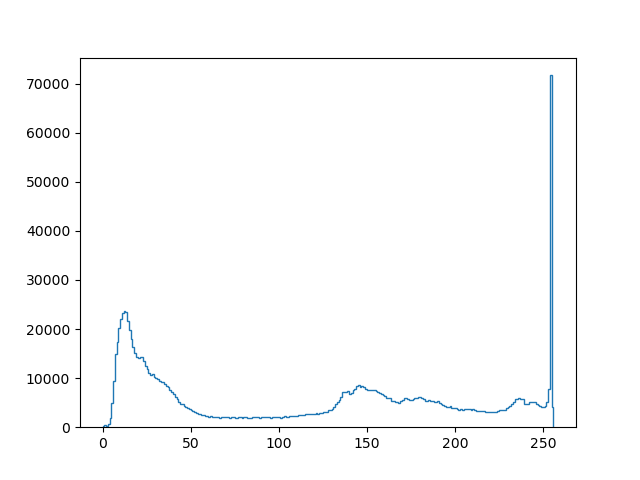
\includegraphics[width=0.5\textwidth]{resources/original_histogram.png}
    \caption{Original histogram plot of the image b1.png}
    \label{fig:plot1}
    \end{figure}

\subsection{Histogram Equalization}
After having the information intensity value distributions, rest was easy. We first computed the cumulative histogram of the image by adding the sum of previous intensity values from the original histogram to each element. Cumulative histogram is different than the original histogram in an important aspect, it gives us a non-decreasing function so we can calculate the equalized intensity values from it. We do this by calculating a coefficient from the intensity range and image size with the bottom formula and multiplying it with corresponding values from the cumulative histogram for each value in the original histogram.

\begin{align}
	s_{k} = round[\frac{L-1}{N\cdot M}\cdot h_{c}\cdot (r_{k})]\label{Histogram equalization coefficient formula}
\end{align}
Where,
\begin{align}
	h_{c}\cdot (r_{k}) = \sum {h(r_{i})}\label{Histogram equalization coefficient formula}
\end{align}

\begin{figure}[]
    \centering
    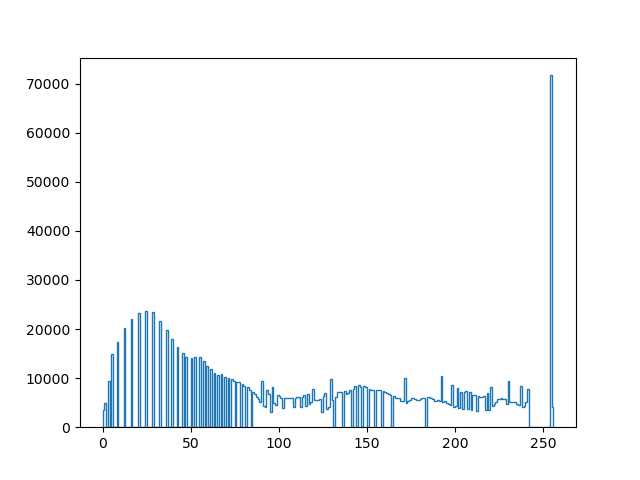
\includegraphics[width=0.5\textwidth]{resources/equalized_histogram.png}
    \caption{Equalized histogram plot of the image b1.png}
    \label{fig:plot2}
\end{figure}

\begin{figure}[]
    \centering
    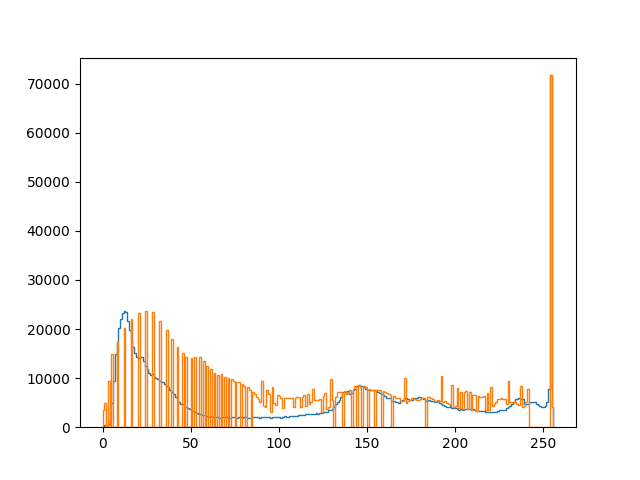
\includegraphics[width=0.5\textwidth]{resources/equalized_histogram_comp.png}
    \caption{Comparison of equalized histogram and original histogram on the same plot b1.png}
    \label{fig:plot3}
\end{figure}


\subsection{Adaptive Histogram Equalization}
Adaptive histogram equalization differs from the histogram equalization by the context they are taking account. Histogram equalization takes the whole image and compute the distributions from all pixels but adaptive histogram equalization works more locally, takes some part of the image into account and only affects that part of the image. This gives us more detail piece wise but to make the final image more visually appealing we need to apply more filtering techniques or change the equalization technique fundamentally. Our image has visible difference lines between the parts that our equalization technique  uses as local areas.

\begin{figure}[]
    \centering
    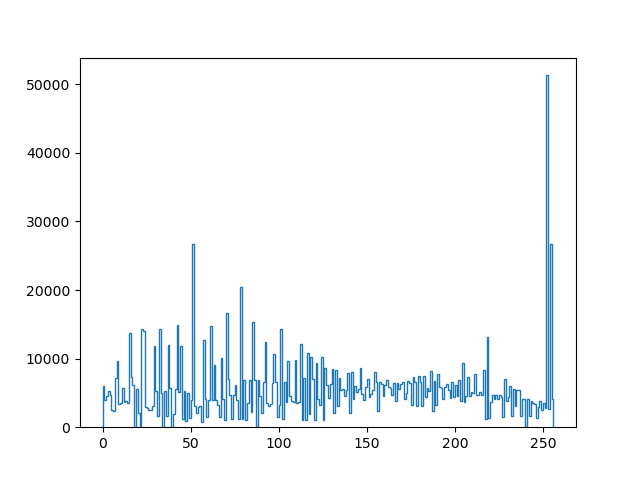
\includegraphics[width=0.5\textwidth]{resources/adaptive_equalized_histogram.png}
    \caption{Adaptively equalized histogram plot of the image b1.png}
    \label{fig:plot4}
\end{figure}

\section{Dependencies}
We used following libraries for the described reasons.
\begin{itemize}
	\item \textit{os:} Handling non-existant input or output paths.
	\item \textit{PIL:} Reading images and converting them arrays.
	\item \textit{numpy:} Executing array and matrix operations.
	\item \textit{math:} Performing trigonometric operations.
	\item \textit{mathplotlib:} Creating histograms as graphics and writing arrays as image files.
\end{itemize}

\end{document}
